% Created 2025-02-27 Thu 15:15
% Intended LaTeX compiler: pdflatex
\documentclass[11pt]{article}
\usepackage[utf8]{inputenc}
\usepackage[T1]{fontenc}
\usepackage{graphicx}
\usepackage{longtable}
\usepackage{wrapfig}
\usepackage{rotating}
\usepackage[normalem]{ulem}
\usepackage{amsmath}
\usepackage{amssymb}
\usepackage{capt-of}
\usepackage{hyperref}
\usepackage[danish, ]{babel}
\usepackage[margin=2.5cm]{geometry}
\usepackage{lmodern}
\usepackage[style=verbose-ibid,backend=bibtex]{biblatex}
\addbibresource{bibliography.bib}
\hypersetup{colorlinks, linkcolor=blue, urlcolor=blue}
\author{Alexander Knudsen, Andreas Jensen og Jeppe Bøgeskov}
\date{\today}
\title{Teknologiprojekt -- Fremtidens levevis}
\hypersetup{
 pdfauthor={Alexander Knudsen, Andreas Jensen og Jeppe Bøgeskov},
 pdftitle={Teknologiprojekt -- Fremtidens levevis},
 pdfkeywords={},
 pdfsubject={},
 pdfcreator={Emacs 29.4 (Org mode 9.7.11)}, 
 pdflang={Dk}}
\begin{document}

\newgeometry{top=2.0cm, bottom=2.0cm}
\begin{titlepage}
    \centering

    \vspace*{1cm}

    % Title and subtitle are enclosed between two rules.
    \rule{\textwidth}{1pt}

    % Title
    \vspace{.7\baselineskip}
    {\huge \textbf{Projekt 1 - Krisen kradser}}

    % Subtitle
    \vspace*{.5cm}
    {\LARGE Efterårssemester 2024}

    \rule{\textwidth}{1pt}

    \vspace{1cm}

    % Set this size for the remaining titlepage.
    \large

    % Authors side by side, using two minipages as a trick.

    \begin{table}[h]
        \centering
        \begin{tabular}{cc}
            \begin{minipage}{.5\textwidth}
                \centering
                Jeppe Bøgeskov Bech \\
                {\normalsize \url{jepp9920@zbc.dk}}
            \end{minipage}
            &
            \begin{minipage}{.5\textwidth}
                \centering
                Alexander Schade Knudsen \\
                {\normalsize \url{alex245h@zbc.dk}}
            \end{minipage}
        \end{tabular}

        \vspace{1cm} % Adds vertical space between the rows

        \begin{minipage}{.5\textwidth}
            \centering
            Andreas Jensen \\
            {\normalsize \url{andr328q@zbc.dk}}
        \end{minipage}
    \end{table}








    % More authors can be inserted here with additional minipages.

    \vspace{1cm}

    % Report logo.
    \fbox{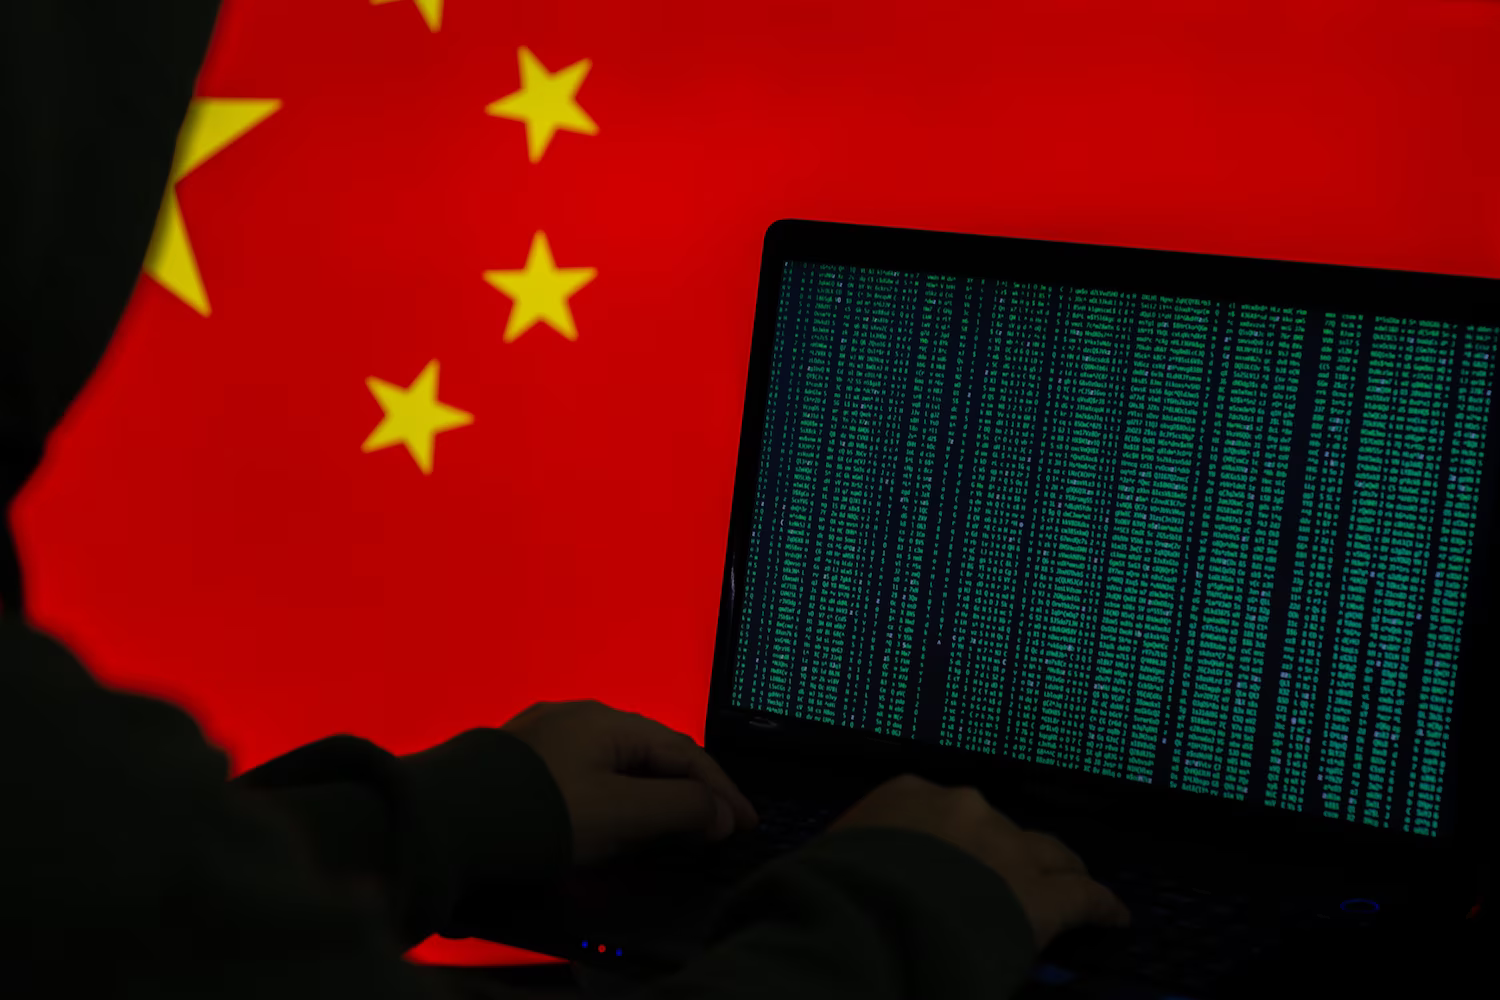
\includegraphics[width=.7\textwidth]{./assets/forsidebillede.png}}

    \vfill

    % University and date information at the bottom of the titlepage.
    2. x \\
    ZBC Handels- og Teknisk gymnasium Slagelse \\
    Akademisk år 2024-2025 \\
    \today
\end{titlepage}


\restoregeometry
\tableofcontents
\newpage
\section{Abstract}
\label{sec:org6419ad8}
In this report, is the work process and descisions leading to creating a smart home system that prioritises data security and self-custody. The report encompases the problem identification, problem analysis, product principles, product realisation and product presentation. The main goal of the product is to create af proof-of-concept smart-home-device that focusses on personal and national security.
\newpage

\section{Indledning}
\label{sec:org6d9531c}
\subsection{Projektstyring}
\label{sec:org5e3ff51}
\subsubsection{Oplæg}
\label{sec:orgbec7f1d}
Heri projektet arbejdes der med casen, der omhandler 'bolig'.
\subsubsection{Tidsstyring}
\label{sec:org730faaa}
\begin{itemize}
\item Startdato: 9. december 2024
\item Slutdato: 11. marts 2025
\end{itemize}
\begin{enumerate}
\item Gantt-diagram
\label{sec:orgb1d2daa}
\end{enumerate}
\subsection{Problemidentifikation}
\label{sec:orgfafb1b0}
Indenfor temaet er der en række forskellige emner, som kunne være relevante at arbejde med, herunder high-tech-løsninger. Grundet gruppens kompetencer, er denne valgt, hvorfor problemidentifikation er afgrænset hertil.
\subsubsection{Samfundsmæssige problemstilling}
\label{sec:orga952bf5}
Mange af de største smart home-løsninger kommer fra udenlandske firmaer, herunder Google, Apple, Amazon, men også firmaer, der er blevet kritiseret meget, såsom TP-Link. \footfullcite{tplink}

Desuden beskrives i sikkerhedsdatablade også, hvordan samtlige IoT-enheder har været anvendt af kinesiske, statssponsorede, hackere, ved at indgå i botnet,\footnote{Et botnet er et netværk af bots (inficerede computermaskiner), som anvendes til synkronangreb mod andre maskiner fx i DDOS-angreb (Distributed Denial of Service).} til at angribe kritiske sektorer i det amerikanske samfund, såsom militær-, udannelseinstitutioner og telekommunikationsløsninger. \footfullcite{securityweek2024chinesespies}

Ifl. Forsvarets Efterretningstjeneste, vurderer Center for Cybersikkerhed, at Ruslands øgede risikovillighed med hensyn til brug af hybride virkemidler mod NATO-lande, herunder Danmark, også omfatter destruktive cyberangreb.\footfullcite{fe-ddis} Indtil videre er der ikke anmeldt angreb via IoT\footnote{IoT er forkortelsen for Internet Of Things, hvilket er en betegnelse for alle teknologier som benytterr sig af diverse internetprotokoller}, men det kan ikke udelukkes, at Rusland, som er allieret med Kina, potentielset ville kunne udnytte Kinesiske firmaers adgang til data iagt af deres markedsandel indenfor IoT.

Grundet, at det Kommunistiske Kinesiske Parti har regeringsmagten i Kina, medfører dette totalitær lovgivning, der muliggør, at partiet kan indkræve samtlige data fra firmaer, der oppererer til lands \footfullcite{securityweek2024chinesespies}. Potentialet i dette alene, er nok til at refærdiggøre udvikling af et alternativt produkt, såsom det, der heri rapporten beskrives.

Således er der få alternativer til status quo, som der herfra kan viderudvikles på. Se afsnit om idegenerering (\ref{sec:org12d3e0c}).
\subsection{Idegenerering}
\label{sec:org12d3e0c}
Alternativerne til status quo-IoT-løsningerne er følgende:
\begin{itemize}
\item Afdigitalisering af nuværende løsninger
\item Udvikling af decentraliserede løsninger, der involverer self-custody (indsæt fodnote)
\item Udvikling af centraliseret løsninger, udgivet af et troværdigt firma i et land, der ikke kræver udleveringen af data fra sine brugere
\end{itemize}
\subsection{Idesortering (lyskurvemetoden)}
\label{sec:orgb65406b}
Den første løsning indebærer, at man bevæger sig væk fra vores oprindelige afgrænsning af fokusområde, nemlig det digitale, hvilket i øvrigt findes i forvejen, hvorfor markedet for dette vurderes mættet.

Desuden grundet gruppens IT-kompetencer, virker de to resterende løsninger som mere kompatible med gruppen. Imellem disse to ideer, vurderes det, at den mere spændende løsning er at lave det decentraliseret med en såkaldt FOSS-løsning, se kapitlet herom (indsæt kapitellink)
\subsection{Afgrænsning}
\label{sec:orgc46d8ef}
Da en total smarthjemsløsning er meget omfattende, vælges der herfor at fokusere på enkelte dele af en sådan løsning. I dette tilfælde er det endelige produkt et proof-of-concept, hvori en smarthub kan sende signaler og modtage signaler til andre eheder på et lokalt netværk. Desuden skal denne kunne fjernbetjenes igennem en styringsapplikation.
\newpage

\section{Problemanalyse}
\label{sec:org3679584}

I problemanalysen er problemstillingen blevet yderligere konkretiseret bl.a. ved et problemtræ (indsæt link til problemtræ)
\begin{figure}[htbp]
\centering
\includegraphics[width=.9\linewidth]{assets/Problemtræ.png}
\caption{Viser projektets problemtræ}
\end{figure}
\subsection{Interessentanalyse}
\label{sec:org976cef3}
\subsubsection{Ekstern interessenter}
\label{sec:orgf2dab0a}
\begin{itemize}
\item NGO'er
\end{itemize}
\subsubsection{Gidsel}
\label{sec:org34c7521}
\begin{itemize}
\item Konsumenter
\end{itemize}
\subsubsection{Grå eminence}
\label{sec:orgaa235ac}
\begin{itemize}
\item Konkurrenter
\end{itemize}
\subsubsection{Ressourceperson}
\label{sec:org63a3f15}
\begin{itemize}
\item Staten
\end{itemize}
\subsection{HV-modellen}
\label{sec:org6b97fc3}
\subsubsection{Hvad}
\label{sec:orgbaa59e1}
\begin{enumerate}
\item Et konkurrencealternativ
\end{enumerate}
\subsubsection{Hvorfor}
\label{sec:orgda4cb7c}
\begin{enumerate}
\item For at få markedsandel på vestlige hænder
\end{enumerate}
\subsubsection{Hvem}
\label{sec:org4e76554}
\begin{enumerate}
\item Et privat firma.
\item Kinesiske firmaer påvirkes, her negativt.
\end{enumerate}
\subsubsection{Hvor}
\label{sec:org442bab2}
\begin{enumerate}
\item Resten af vestlige lande.
\end{enumerate}
\subsubsection{Hvordan}
\label{sec:org66417d5}
\begin{enumerate}
\item Decentralt IoT-system
\end{enumerate}

\newpage
\section{Produktprincip}
\label{sec:orga77d6f9}
\subsection{Målgruppe}
Et værktøj til at beskrive sin målgruppe inden for teknologifaget, er at lave en persona. Dette gøres for at det kan vises et fiktivt eksempel på en person som kunne have interesse for at købe produktet.

\textbf{Køn}: Mand

\textbf{Alder}: 34

\textbf{Beskæftigelse}: Revisor

\textbf{Status}: Gift

\textbf{Bopæl}: Herlev

\textbf{Interesser}: 
\begin{itemize}
\item Fisker
\item Finans
\item Teknologi
\end{itemize}

\textbf{Teknologisyn}: 
\begin{itemize}
\item Smarte hjem
\item Android-bruger
\end{itemize}

Dette vil sige at personen er interesseret i at have et smart hjem, og ikke har alverdens tid til at lave en lignende løsning selv.

\subsection{Kravspecifikation}
\label{sec:kravspecifikation}
Her opsættes kravspecifikationen for smarthjem-systemet (specifikt smart-gardin-systemet \ref{sec:orgc46d8ef}).
\begin{itemize}
\item Gardinet skal kunne kontrolleres fra en smartphone
\item Styreingen skal ske trådløst
\item Styringen skal være nemt at benytte (Som en fjernstyring)
\item Produktet skal have en rimelig pris
\item Enheden skal fungere via intranet (dvs. produktet skal virke i et lokalt netværk)
\item FOSS \ref{sec:loesningsforslag}
\end{itemize}


\subsection{Konkurrentanalyse}
\label{sec:konkurrentanalyse}
\subsubsection{IKEA}
IKEA leverer IoT-produkter, som f.eks. smarte lamper, stik samt smart-rullegardiner. Fordelen ved IKEAs produkter er, at de er relativt billige sammenlignet med andre produkter på markedet, at de indgår i et veludviklet og etableret smart-økosystem samt at de er lette at installere.
IKEAs produkter bliver fremstillet af tvangsarbejdere af bla. hviderussiske fanger. \footfullcite{IKEA} grudnet geopolitiske omstændigheder kan det være problematisk at produkterne bliver fremstillet i Hviderusland.\Ref{sec:orga952bf5}
\begin{figure}[htbp]
\centering
\fbox{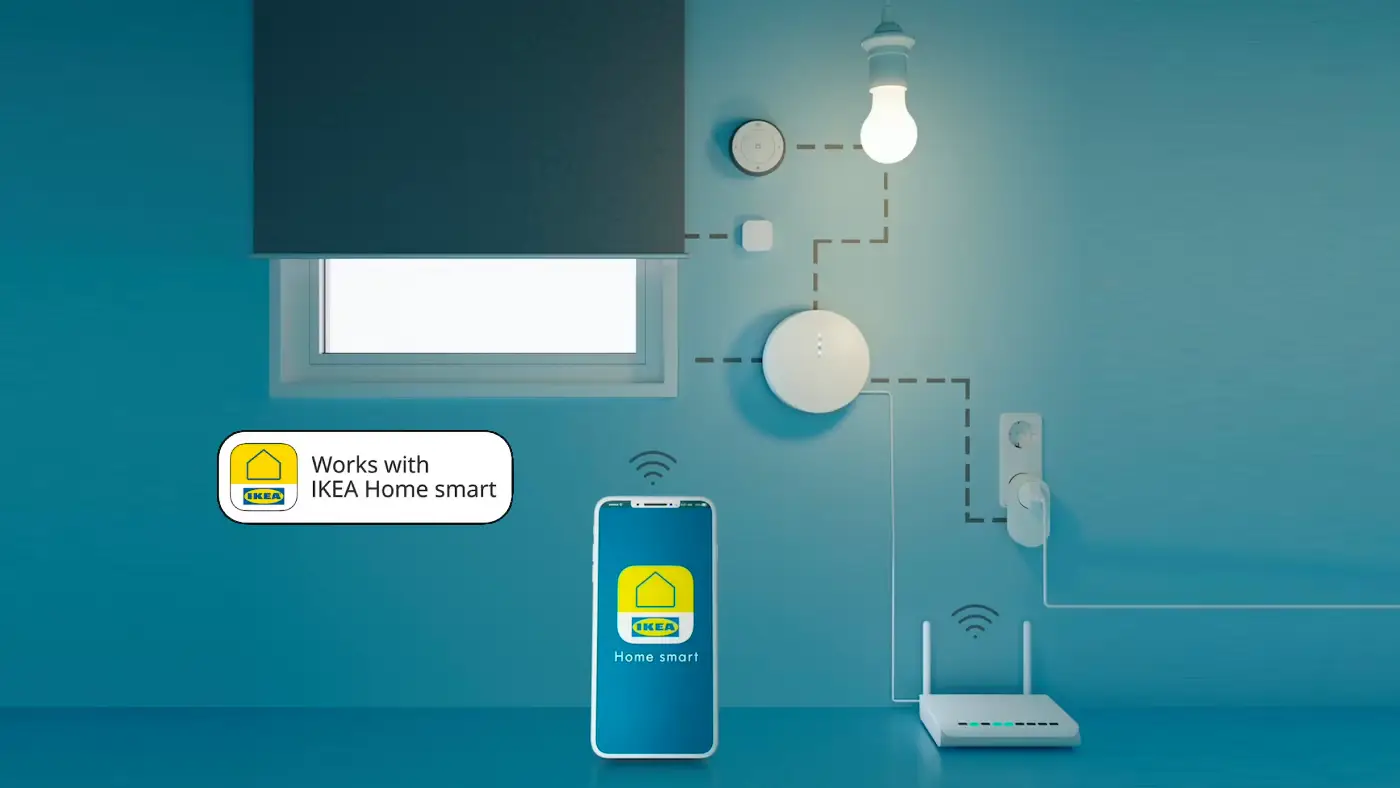
\includegraphics[width=.75\linewidth]{assets/Ikea-smart-home.png}}
\caption{Viser en illustration af IKEA smart-home}
\end{figure}
\subsubsection{TP-Link}
Problematikkerne vedrørende TP-Link er tideligere blevet beskrevet i afsnit \ref{sec:orga952bf5}.
\subsubsection{Xiaomi}
Xiaomi er et kinesisk firma, der leverer en lang række smart-hjemme-produkter med et meget stort udvalg. Fordelene ved Xiaomi er, at brugeren kan købe alle smart-hjem-produkterne under ét firma, hvilket gør det lettere at kontrollere, da de bruger en samlet platform til at styre alle deres produkter. Ulempen ved Xiaomi er, at det er et Kinesisk firma, hvilket udgør en stor risiko\ref{sec:orga952bf5}. Produkterne fra Xiaomi er også relativt billige sammenlignet med andre mere premium produkter på markedet.

\begin{figure}[htbp]
\centering
\fbox{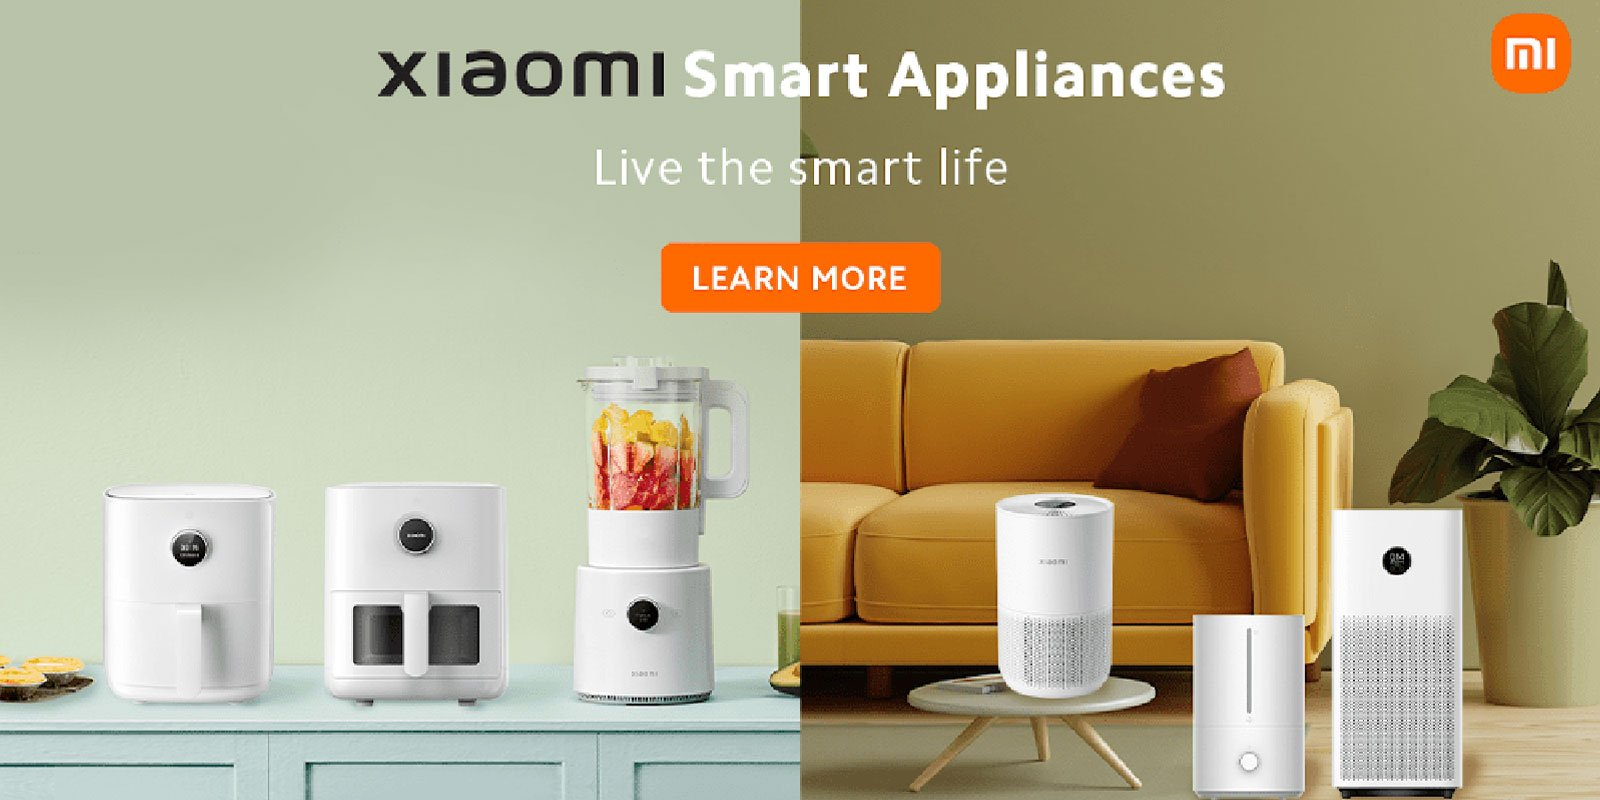
\includegraphics[width=.75\linewidth]{assets/xiaomi.jpg}}
\caption{Viser en illustration af Xiaomi smart-home}
\end{figure}

\subsubsection{Huawei}
Huawei er også en kinesisk virksomhed, som blandt andet udbyder en række smart-produkter. Det må siges at virksemheden her passer lige ind i den overordnede samfundsmessige problemstilling \ref{sec:orga952bf5}, hvor it-sikkerheden omtales da den amerikanske start har valgt at banlyse salg og import af nye huawei-produkter. Dette gjorde staten fordi at de frygtede der var en risiko for såkaldte "bagdøre" (backdoors) i virksomhedens produkter.\footfullcite{huawei}
\begin{figure}[htbp]
\centering
\fbox{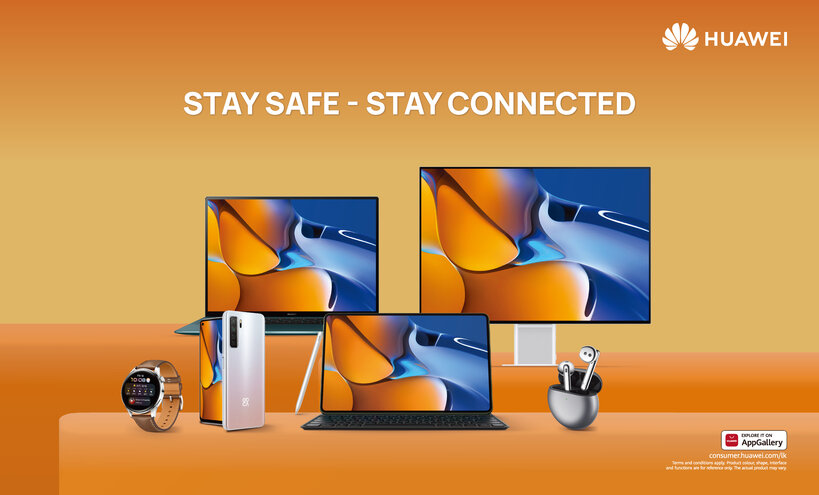
\includegraphics[width=.75\linewidth]{assets/huawei.jpg}}
\caption{Viser en illustration af Huawei smart-home}
\end{figure}

\subsection{Løsningsforslag}
\label{sec:loesningsforslag}
\subsubsection{Software}
Softwaren skal udvikles efter FOSS-princippet, hvilket betyder at softwaren skal være frit tilgængelig for alle, kan viderudvikles og distribueres frit. Dette er med til at understøtte princippet om decentralisering og gennemsigtighed, som virksomheden bygger på. Det skaber også en større sikkerhed for brugeren, da tech-nørder kan gennemse kildekoden og tilføje forbedringer til softwaren samt råbe vagt i gevær såfremt der er tale om en sikkerhedsrisiko. Desuden vil en softwareudvikler også være tilknyttet projektet, fuld- eller deltids, afhængigt af arbejdsbyrden. Koden skal synkroniseres med GitHub. Git skal anvendes til udviklig- og versionshåndtering.

\subsubsection{Finansiering}
\label{sec:finansiering}
For at produktet bliver konkurrencedygtigt, er det nødvendigt, at prisen herpå sænkes (se konkurrenceanalyse \ref{sec:konkurrentanalyse}). Det kunne her tænkes, at staten ville være interesseret i at medfinansiere projektet, herunder subsidierer produktet delvist, da dette vil kunne give større markedsandel til et indlandsfirma, som er troværdigt og hvis sikkerhedsrisci er færre og mindre; hvilket kan være vigtigt for den danske sikkerhedspolitiske situation.
\newpage

\section{Produktudformning}
\label{sec:org563ee9e}
I Idegenereringsfasen blev dedigitaliseringen af smart-hjem-produkter som der finde på markedet omtalt, derfor har vil er det beslutet at der skal udvikles et smart-rullegardin som følger kravene i kravspecifikationen\ref{sec:kravspecifikation} og som derved sikre brugerens data og privatliv fra fjentligtsindede magter omkring i verden.
% Under idegeneringen blev der talt om at dedigitalisere de smart-hjem-produkter som der findes på markedet, derfor har vi tænkt os at designe og udvikle et smart-hjem-rullegardin som brugeren kan kontrollere fra sin smartphone, dette fjerner risikoen med at brugerens data bliver lagret og solgt til virksomheder omkring i verden.

\subsection{Hardware}
\label{sec:orgdbd4fd8}
\subsubsection{3D-print}
Vi besluttede os for at det mest praktiske og realistiske materiale til at producere vores prototype i ville være plastik, altså en 3D-printet kasse hvor vi kan have vores elektroniske komponenter. Her besluttede vi os for at printe med PLA-Plastik da dette er et billigt og forholdsvist holdbart materiale. En anden grund til at vi besluttede os for at benytte en 3D-printet kasse er at det er hurtigt at iterere og forbedre dit design, og det er et ikke særligt dyrt materiale, hvilket gør det økonomisk bevidst at benytte dette til prototypen.
\begin{figure}[htbp]
    \centering
    \fbox{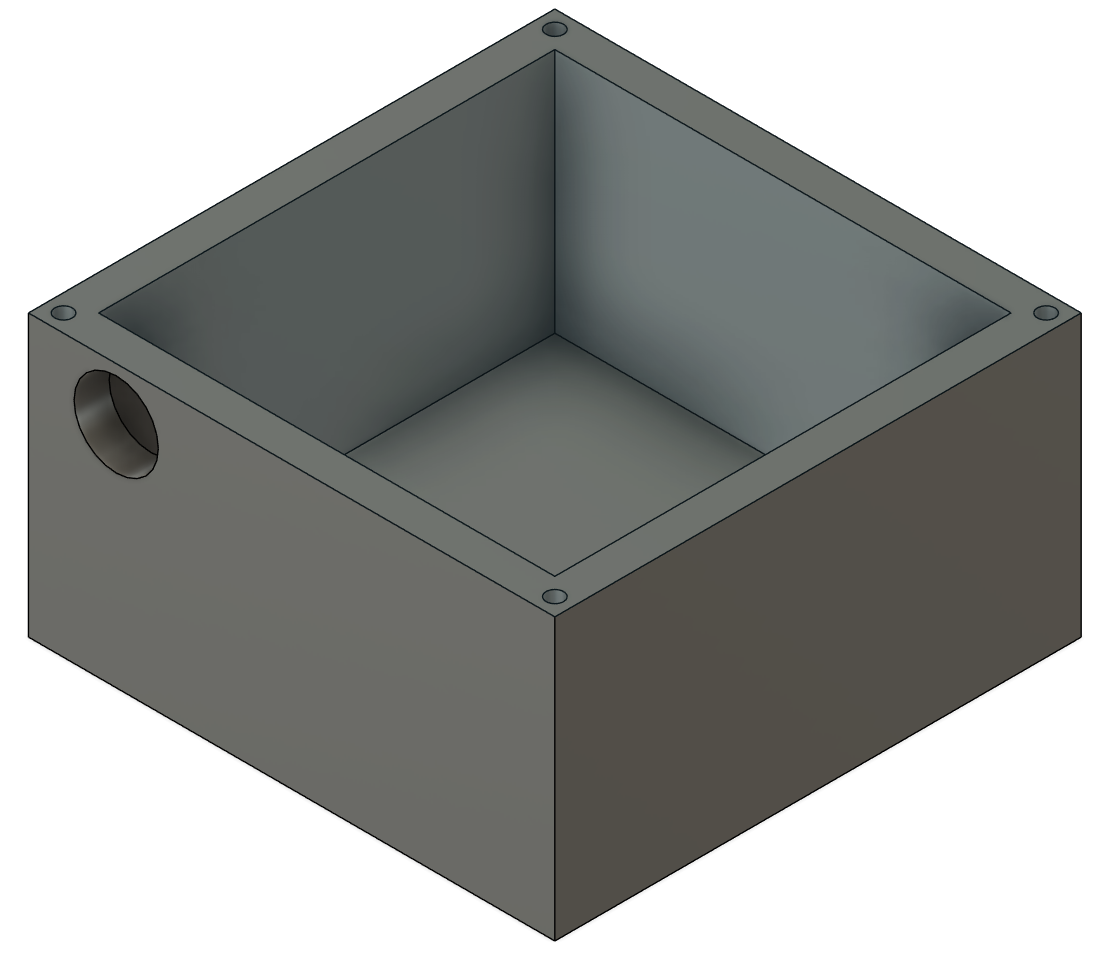
\includegraphics[width=.75\linewidth]{assets/Kasse.png}}
    \caption{Viser en Fusion360 3D-tegning af Kassen}
    \end{figure}
Kassen er simpel da fokuset ikke var at skabe noget der var pænt til at starte med, den er derimod meget funktionel da den gør det muligt at komme til alle individuelle komponenter. Der er også et hul i siden af kassen som er tilpasset til en 12v DC motor, dette gør så at motoren kan sidde fast monteret i kassen. De fire huller i toppen af kassen er lavet så et låg kan monteres for at skjule og beskytte elektronikken i kassen.

\begin{figure}[htbp]
    \centering
    \fbox{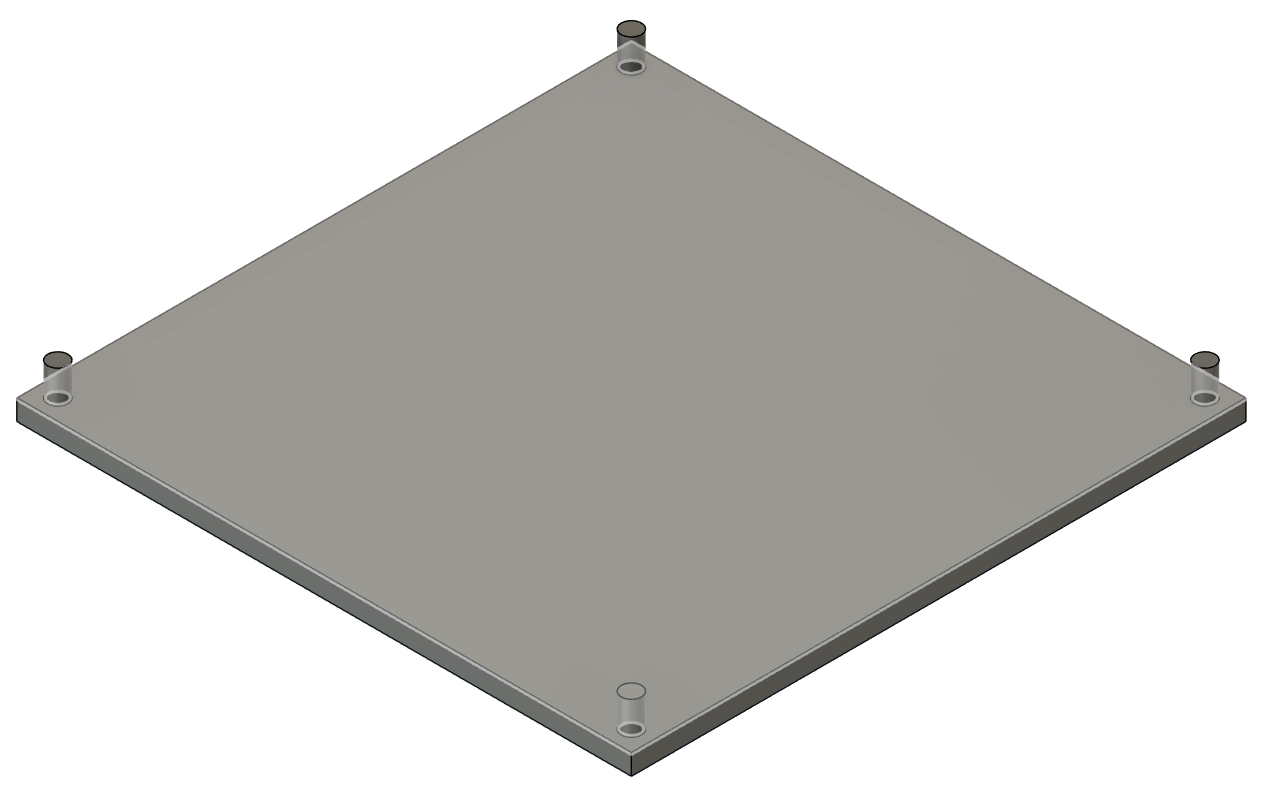
\includegraphics[width=.75\linewidth]{assets/Lag.png}}
    \caption{Viser en Fusion360 3D-tegning af Låget}
    \end{figure}

Den sidste ting som vi har 3D-printet i forbindelse med vores produkt er et montage stykke til motoren. Det er en cirkel hvor motorens aksel passer i midten. Dette gør det muligt for motoren at dreje rundt på vores gardinstang, da det er muligt at benytte samme teknik som vi har brugt til montage stykket på en roterende gardinstang.

\begin{figure}[htbp]
    \centering
    \fbox{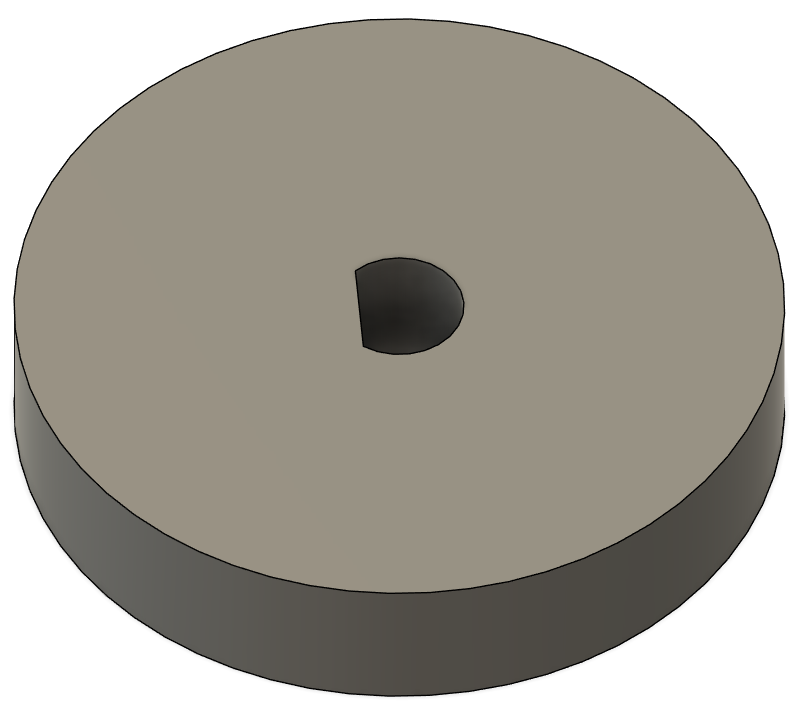
\includegraphics[width=.4\linewidth]{assets/Montage-Stykke.png}}
    \caption{Viser en Fusion360 3D-tegning af Montage-Stykket}
    \end{figure}

Den kasse som vi endte ud med opfylder alle de krav som vi stilte, den er nem og billig at producere, og den holder vores elektronik sikkert og samlet. 

\begin{figure}[htbp]
    \centering
    \fbox{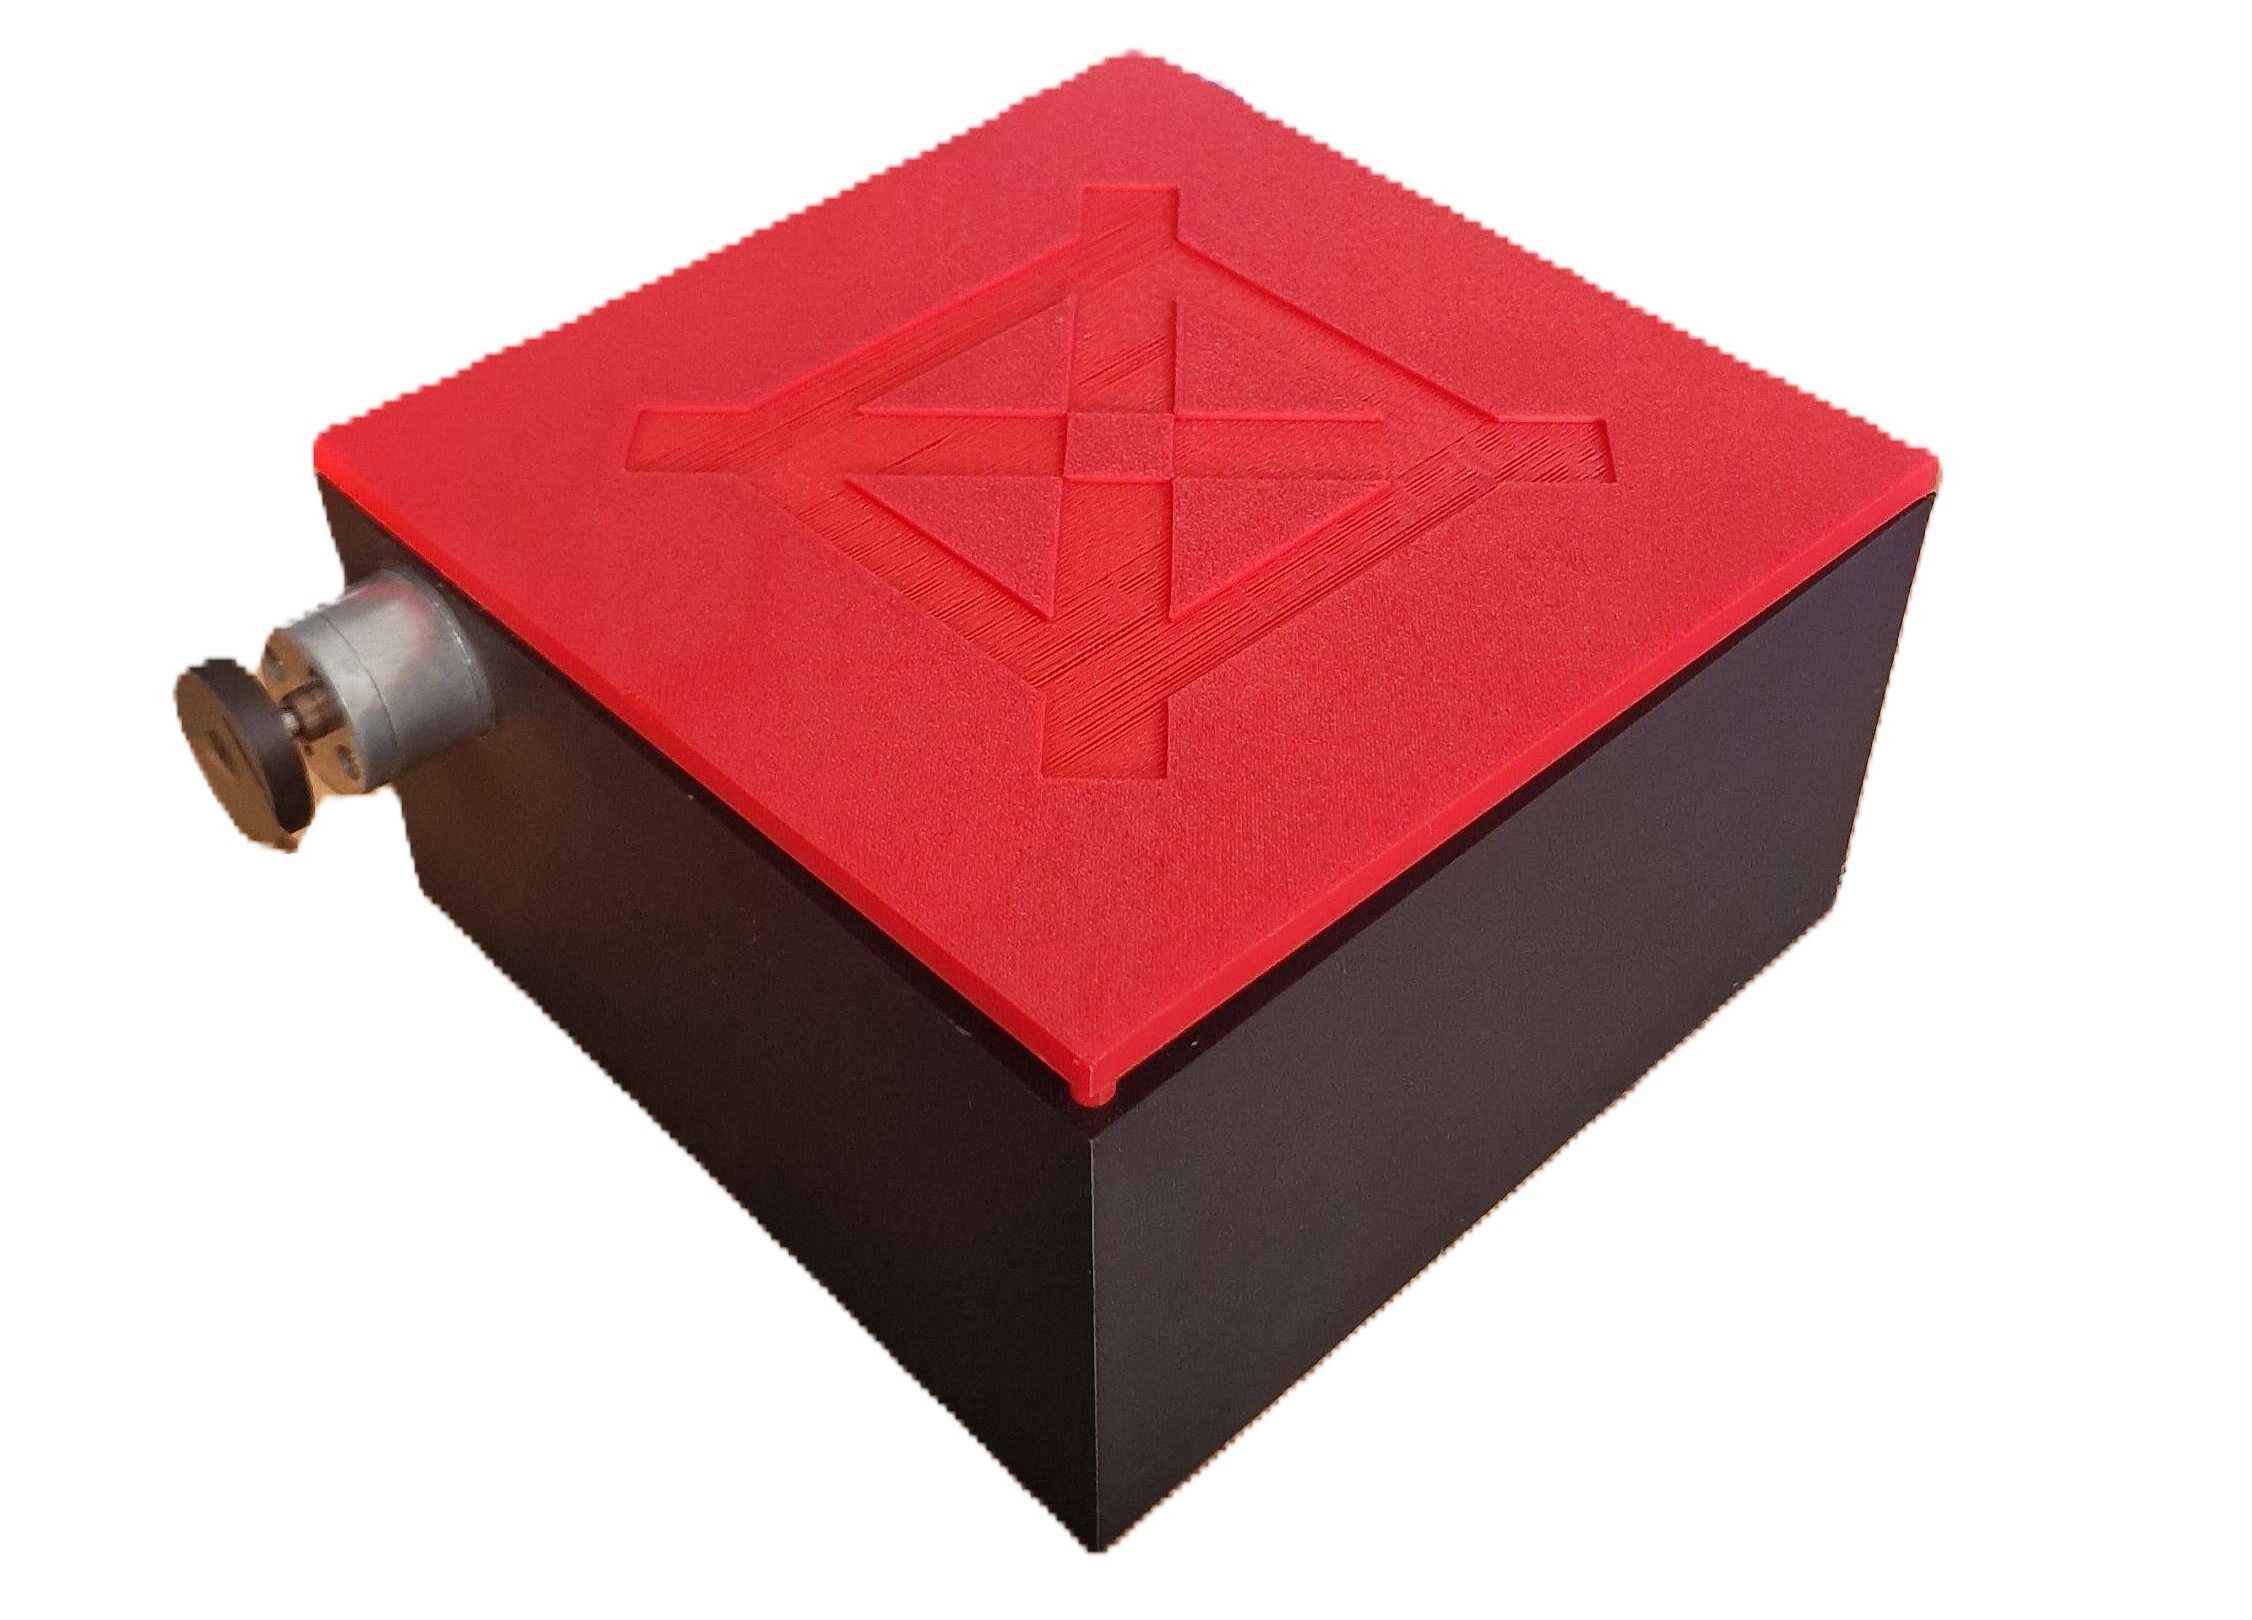
\includegraphics[height=.55\linewidth]{assets/Kasse-frdig.png}}
    \caption{Her ses den endelige udgave af produktet. }
    \end{figure}

\subsubsection{Elektronik}
I elektronik delen var der nogle også krav der skulle opfyldes, elektronikken skal på sigt kunnes optimeres med special-designede PCB'er. Elektronikken skal også gøre det muligt at bruge WIFI funktionen som vores projekt bygger på.

\begin{figure}[htbp]
    \centering
    \fbox{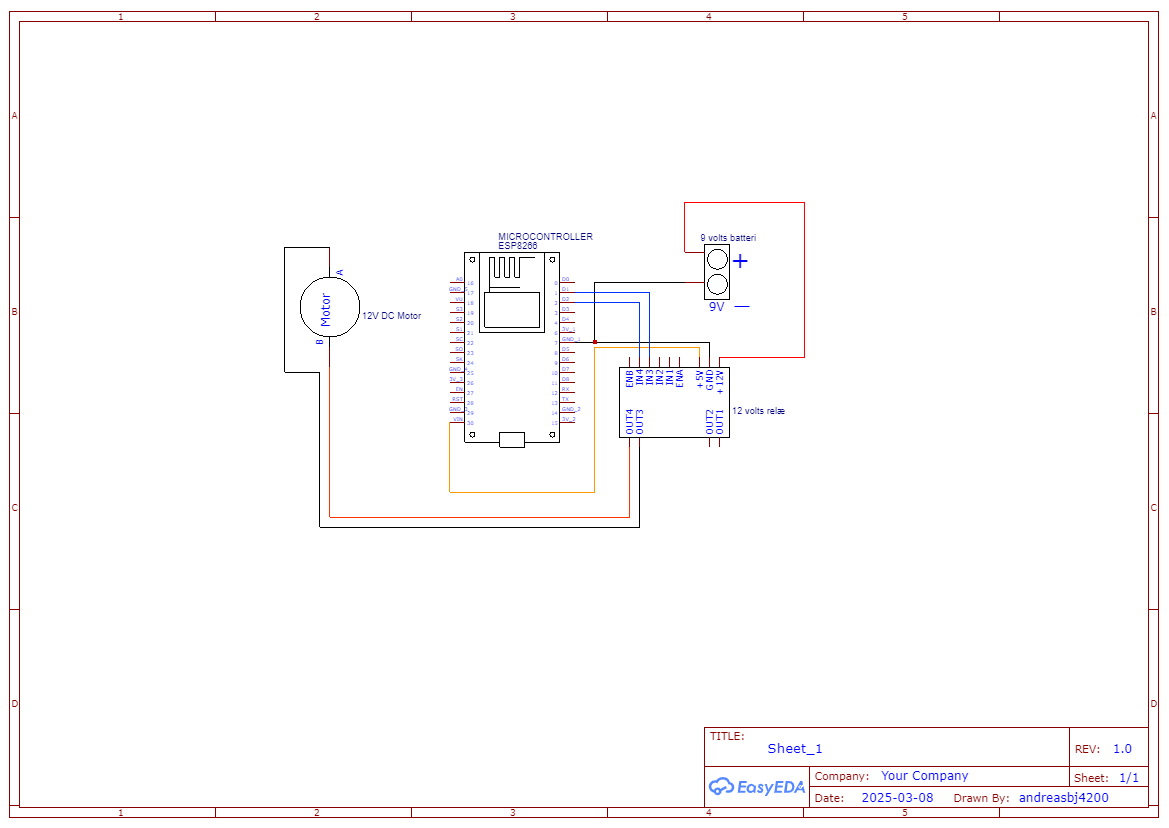
\includegraphics[width=.75\linewidth]{assets/EL-diagram.png}}
    \caption{Her ses EL-digrammet, tegnet i EasyEDA. }
    \end{figure}

Elektronik delen var forholdsvist ligefrem da vi vidste at vi skulle have en Microcontroller med WIFI indbygget. Her valgte vi at bruge en ESP8266MOD da de er nemme at programmere takket være ArduinoIDE's ESP8266 Bibliotek. Som også kan ses på billedet ovenfor, benytter vi os af et 9 volts batteri selvom at vi bruger en 12 volts DC motor. Dette er for nemmere at kunne styre den hastighed som motoren kører med, og de 9 volt er stadig rigeligt til at trække motoren, og give strøm til vores ESP8266.


\subsection{Software}
Det er essentielt for vores produkt af vores microcontrollers kan fungere over WIFI, til dette har vi benyttet ArduinoIDE's indbyggede ESP8266 bibliotek da dette giver muligheden for at koble din ESP8266 på WIFI, og på den måde kontrollere den fra vores Smartphone.

\section{Produktionsforberedelse}
\label{sec:orge880538}

\subsection{Masseproduktion}
\label{sec:orge66eada}
\section{{\bfseries\sffamily TODO} Evaluering}
\label{sec:org4ddb451}
\subsection{Hardwarepåvirkning}
\label{sec:org9e89a3f}
\subsection{Softwarepåvirkning (serverpåvirkning)}
\label{sec:org15c2cb6}

\newpage
\section{Miljøvurdering}
\label{sec:miljoevurdering}
\subsection{Forurening i produktionsøjemed}
Den primære udledning af CO2, som direkte konsekvens af produktet heri beskrevet, vil kunne ses i produktionsøjemed.
\subsection{Forurening i privaten dvs. under anvendelse}
Ligedan vil der udledes CO2 ifbm. energiskabelse til disse enheder. Det forventes dog i første omgang, at markedsandelen vil være lille, at produkterne vil kunne produceres on-demand og at det iøvrigt er et alternativ til andre smarthjemløsninger, som folk ellers havde købt.
\subsection{Forurening ifbm. med fragt}
Logistik ifbm. tidlig on-demand produktion kan medregnes i distribuantens CO2-regnskab, men skal sidenhen revideres i opskalering af produktion. 

\newpage
\section{Konklusion}
\label{sec:org7454aed}
Projektet er kulmineret i et proof-of-concept, som viser, at det er muligt at lave et smat-hjem-system, som er decentraliseret og kan være sikkert (såfremt der ikke var en evt. bagdør i ESP-32'en). Selve produktet er en anelse defekt, idet der ikke var taget højde for printersporene på de 3D-printede knobber, der udgør lukkemekanismen på kasen, som indeholder maskineindmaden.

Projektets kulmination kunne have været mere elaborat havde tiden hertil været bedre spenderet og projektet bedre koordineret. Desuden er projektet undervejs blevet udsat for en række forsinkelser, herunder sygdom, hvorfor nogle tråde undervejs har skulle gensamles. Dette er uundgåeligt og har således også givet en lærestreg i vigtigheden af at have en god plan, med færdige mål og opgaver, personspecifikt og på forhånd.

\newpage
\printbibliography
\end{document}
2